\chapter{Arbeitsumgebung}\label{ch:arbeitsumgebung}
In diesem Abschnitt wird der Arbeitsplatz und die Umbgebung, während der Probe-IPA, des Kandidaten beschrieben.
\section{Arbeitsplatz}\label{sec:arbeitsplatz}

\begin{figure}[H]
    \begin{center}
        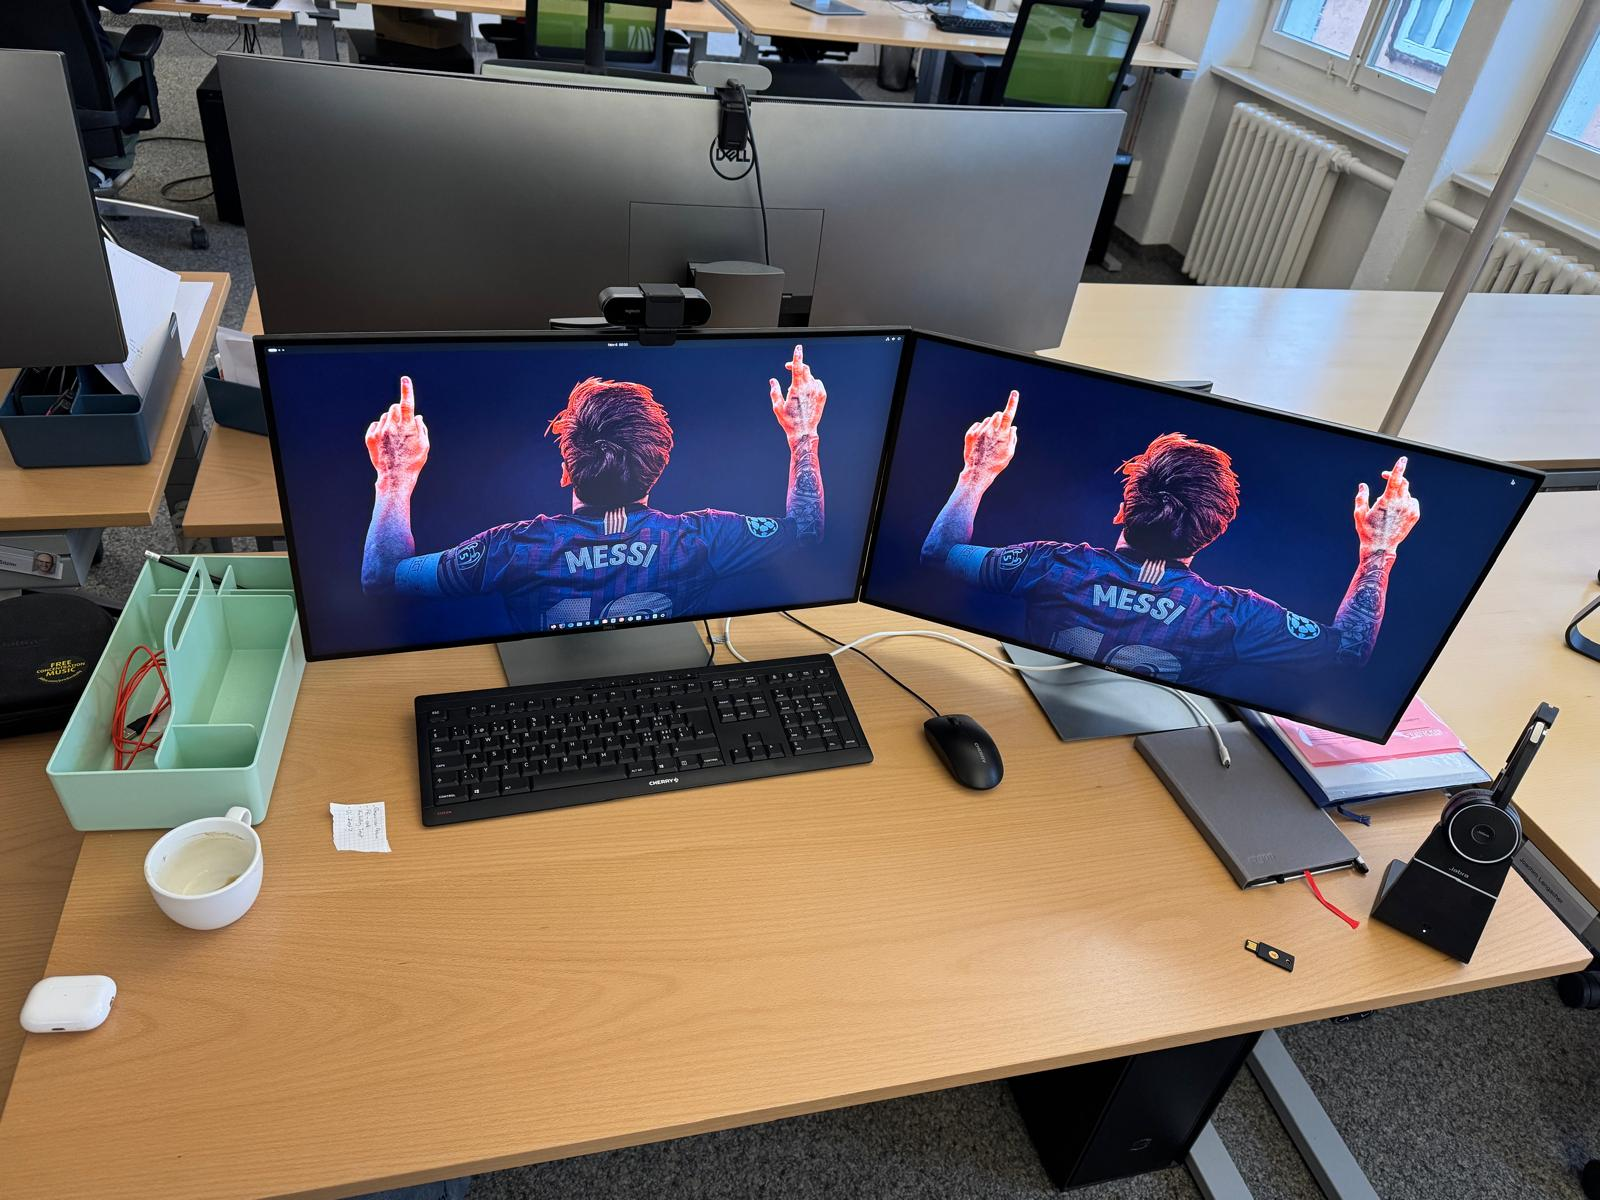
\includegraphics[width=0.8\textwidth]{ressourcen/arbeitsplatz}
        \caption[Arbeitsplatz]{Arbeitsplatz während der Probe-IPA}\label{fig:arbeitsplatz}
    \end{center}
\end{figure}

Da seit der Mitarbeit im IAM nie im Homeoffice gearbeitet wurde, findet auch die Probe-IPA wie gewohnt vor Ort statt. Der Desktop PC mit dem Betriebssystem Linux (Distribution Ubuntu) ist für die maximale Effizienz mit 2 Bildschirmen verbunden. Um im Grossraumbüro möglichst ungestört zu arbeiten, liegen dem Kandidaten ein Paar Airpods Pro mit Noise Cancelling vor.

\newpage \section{Verwendete Tools}\label{sec:verwendete-tools}
Die folgende Tabelle zeigt einen Überblick der wichtigsten Tools, welche für die Umsetzung der Probe-IPA verwendet wurden:

\renewcommand{\arraystretch}{1.5}
\begin{longtable}{|p{.22\textwidth}|p{.40\textwidth}|p{.38\textwidth}|}
    \hline
    \textbf{Tool} & \textbf{Einsatzzweck} & \textbf{Link} \\ \hline
    Intellij Ultimate           & Entwicklungsumgebung, zur Entwicklung des Features                   & \url{https://www.jetbrains.com/de-de/idea/}     \\ \hline
    TeXstudio           & Enticklungsumgebung für Latex, mit welchem die Dokumentation geschrieben wurde & \url{https://www.texstudio.org/}     \\ \hline
    Gerrit           & Quellcode Verwaltung & \url{https://www.gerritcodereview.com/}     \\ \hline
    Git          & Versionskontrollsystem & \url{https://git-scm.com/}     \\ \hline
    Jenkins & Automatisierte Testruns  & \url{https://www.jenkins.io/}     \\ \hline
    Outlook & Termin für den Expertenbesuch im Blick behalten& \url{https://www.microsoft.com/de-ch/microsoft-365/outlook} \\ \hline
    Postman & Testen der eigenen API und der API von Futurae & \url{https://www.postman.com/} \\ \hline
    LibreOffice & Erstellen und warten des Zeitplans & \url{https://de.libreoffice.org/} \\ \hline
    Github & Backup und Versionierung des Berichts und des Zeitplans & \url{https://github.com/} \\ \hline
    Gliffy & Diagramme erstellen & \url{https://www.gliffy.com/} \\ \hline
    Mockito & Mocking für Unit-Tests& \url{https://site.mockito.org/} \\ \hline
    JUnit5 & Testframework für Java & \url{https://junit.org/junit5/} \\ \hline
    Selenium & Framework für automatisierte Softwaretests von Webanwendungen  & \url{https://www.selenium.dev/} \\ \hline
    Wiremock & Simulieren des Futurae Server für Unittests & \url{https://www.wiremock.io/} \\ \hline    
\end{longtable}
\renewcommand{\arraystretch}{1}
\newpage